\section{Additional results (exploratory)}
\label{app:results}

\subsection{Other candidate explanations}
\paragraph{History length: weaker, aggregation-dependent evidence.} If
B-EQ needed a long history to represent the distribution of changes, the
gap should shrink for short histories. It does only when scores are
pooled over origins, which weights the accounts with large errors more.
Under the planned account mean, B-EQ keeps a clear long-horizon advantage
with under a year of history, on both splits:

\begin{center}\footnotesize
\begin{tabular}{lll}
\toprule
V2 vs B-EQ, pooled (account mean) & under 12 months & 24 months or more\\
\midrule
Development, \hB\ d & \pq{xd/s3-history-lt12/V2-vs-B-EQ}{30} & \pq{xd/s3-history-ge24/V2-vs-B-EQ}{30}\\
Development, \hC\ d & \pq{xd/s3-history-lt12/V2-vs-B-EQ}{90} & \pq{xd/s3-history-ge24/V2-vs-B-EQ}{90}\\
Held-out, \hB\ d & \pq{xh/s3-history-lt12/V2-vs-B-EQ}{30} & \pq{xh/s3-history-ge24/V2-vs-B-EQ}{30}\\
Held-out, \hC\ d & \pq{xh/s3-history-lt12/V2-vs-B-EQ}{90} & \pq{xh/s3-history-ge24/V2-vs-B-EQ}{90}\\
\bottomrule
\end{tabular}
\end{center}

At \hC\ days the gap is largest at 12--23 months, not at the longest
histories, under both aggregations and on both splits. Whether
B-EQ's advantage depends on the number of past windows is therefore not
settled by these data.

\paragraph{Simulation: schedule regularity, not sparsity.} We crossed four
levels of spending sparsity, from \R{xd/s4/0/0/V2-vs-B-EQ/30/mean_count} down
to \R{xd/s4/3/0/V2-vs-B-EQ/30/mean_count} purchases a day, with four levels
of schedule regularity. The regularity factors are pay-date jitter,
paycheck amount noise and bill drift. Figure~\ref{fig:grid} shows the
result:
\begin{itemize}
\item \textbf{Regular schedules:} V2 has lower CRPS than B-EQ at every
  sparsity, including the sparsest
  (\R{xd/s4/3/1/V2-vs-B-EQ/30/skill_pooled} at \hB\ days).
\item \textbf{The most irregular level:} B-EQ wins at every sparsity
  (\R{xd/s4/3/3/V2-vs-B-EQ/30/skill_pooled} in the sparsest cell).
\item \textbf{Sparsity alone} shrinks V2's lead but never reverses it.
\end{itemize}
In our generator, B-EQ's advantage at \hB\ and \hC\ days needs irregular
schedules. On Berka, the predictability tertiles give only weak support for
the same pattern. The simulation covers \hB\ and \hC\ days
only, and varies the three regularity factors together.

\begin{figure}[t]
\centering
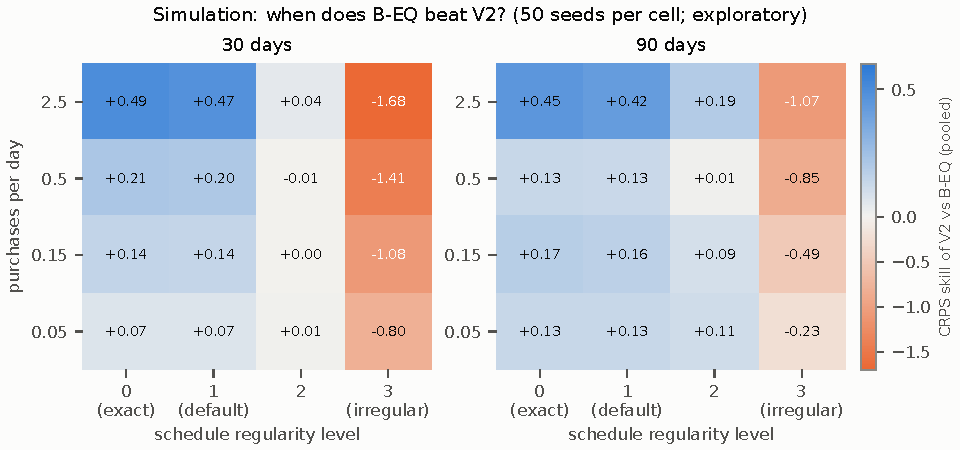
\includegraphics[width=0.85\linewidth]{figures/grid-synthetic.pdf}
\caption{Simulation (exploratory): pooled CRPS skill of V2 against B-EQ by
spending sparsity and schedule regularity, \R{xd/s4/0/0/V2-vs-B-EQ/30/accounts}
seeds and \R{xd/s4/0/0/V2-vs-B-EQ/30/forecasts} origins per cell and
horizon. Blue: V2 has lower CRPS; orange: B-EQ does. Seed-bootstrap
intervals are in \texttt{paper/results/exploratory/s4-grid/}.}
\label{fig:grid}
\end{figure}

\paragraph{Calendar alignment and sparse event counts, as tested.}
\begin{itemize}
\item \textbf{Calendar alignment.} The one rule we tested, restricting
  B-EQ's past windows to those starting within \R{c/cal-half} days of the
  origin's day of the month, makes it slightly \emph{worse} on both splits
  (Table~\ref{tab:explain}). It also leaves B-EQ fewer windows, so it does
  not rule out other forms of calendar alignment.
\item \textbf{Sparse event counts.} Modelling spending as sparse discrete
  events without the filter (CP-noKF) loses to B-EQ by about as much as V2
  does. In our generator, over the sparsity range tested
  (\R{xd/s4/0/0/V2-vs-B-EQ/30/mean_count} to
  \R{xd/s4/3/0/V2-vs-B-EQ/30/mean_count} purchases a day), sparsity alone did
  not give B-EQ the advantage. The filter itself helps a little: removing
  it (CP-noKF against V2) raises CRPS slightly on both splits.
\end{itemize}

\paragraph{Origin phase.} The size of the \hB-day gap depends on where
in the month the origins fall. On development accounts, on grids shifted
by +10 and +20 days, V2's pooled skill against B-EQ is
\R{xd/s8-offset10/V2-vs-B-EQ/30/skill_pooled} and
\R{xd/s8-offset20/V2-vs-B-EQ/30/skill_pooled} (account mean
\R{xd/s8-offset10/V2-vs-B-EQ/30/skill_mean} and
\R{xd/s8-offset20/V2-vs-B-EQ/30/skill_mean}), against
\R{xd/s3/V2-vs-B-EQ/30/skill_pooled}
(\R{xd/s3/V2-vs-B-EQ/30/skill_mean}) on the frozen grid. The sign holds on
every grid.


\subsection{The predictability score}
\label{app:predictability}
For an origin $t$, the checkpoints are $c_j = t - \R{c/pred-step}\,j$ for
$j = 1, \dots, \R{c/pred-checkpoints}$, keeping those at least
\R{c/pred-minhist} days after the account's first record. At each
checkpoint:
\begin{itemize}
\item the records through $c_j$ are tagged and the schedule is detected
  from them alone;
\item the projected events over $(c_j, c_j + \R{c/pred-step}]$ are the
  detected paydays at the latest paycheck's amount and the detected bills'
  due dates at their amounts (overdue ones on the next day), as in B-SR's
  projection;
\item the realized events are the records in the same interval whose
  counterparty (operation, symbol, bank, account) is one of the streams
  detected at $c_j$.
\end{itemize}
With $P_j$ and $R_j$ the projected and realized net flows, the score is
$A = \sum_j |R_j - P_j| / \sum_j |R_j|$. Amounts are in the origin's
normalized units, but $A$ is a ratio and unit-free. A detected stream that
books nothing contributes its projection to the error; a stream not
detected at $c_j$ does not count at all, and neither does timing within the
interval. Origins with fewer than \R{c/pred-minchk} checkpoints or no
realized scheduled flow are unrated
(\R{xh/s17/comp/unrated/origins} held-out origins). The tertile cut points,
fixed from the development distribution, are $A \le \R{xd/s11cut/1-3}$
(predictable) and $A > \R{xd/s11cut/2-3}$ (unpredictable). Matching
projected and realized events within $\pm\R{c/pred-match}$ days gives the
date error and the missed and extra rates, which we report as descriptions
(\texttt{s11-schedule/strata.csv}) and do not use for the tertiles.

\subsection{Shortfall events over all origins and below the tenth percentile}
\begin{table}[t]
\centering\scriptsize\setlength{\tabcolsep}{3.5pt}
\begin{tabular}{ll r rrrrr}
\toprule
Event & $h$ & prevalence (\%) & V2 & CP-noKF & B-EQp & B-SRp & CLIM\\
\midrule
below 0 & \hA & \R{xh/s5/u0/7/prevalence} {\scriptsize(\R{xd/s5/u0/7/prevalence})} & \R{xh/s5/u0/7/brier_V2} & \R{xh/s5/u0/7/brier_CP-noKF} & \R{xh/s5/u0/7/brier_B-EQp} & \R{xh/s5/u0/7/brier_B-SRp} & \R{xh/s5/u0/7/brier_CLIM}\\
 & \hB & \R{xh/s5/u0/30/prevalence} {\scriptsize(\R{xd/s5/u0/30/prevalence})} & \R{xh/s5/u0/30/brier_V2} & \R{xh/s5/u0/30/brier_CP-noKF} & \R{xh/s5/u0/30/brier_B-EQp} & \R{xh/s5/u0/30/brier_B-SRp} & \R{xh/s5/u0/30/brier_CLIM}\\
 & \hC & \R{xh/s5/u0/90/prevalence} {\scriptsize(\R{xd/s5/u0/90/prevalence})} & \R{xh/s5/u0/90/brier_V2} & \R{xh/s5/u0/90/brier_CP-noKF} & \R{xh/s5/u0/90/brier_B-EQp} & \R{xh/s5/u0/90/brier_B-SRp} & \R{xh/s5/u0/90/brier_CLIM}\\
\addlinespace
below own tenth pct. & \hA & \R{xh/s5/u10/7/prevalence} {\scriptsize(\R{xd/s5/u10/7/prevalence})} & \R{xh/s5/u10/7/brier_V2} & \R{xh/s5/u10/7/brier_CP-noKF} & \R{xh/s5/u10/7/brier_B-EQp} & \R{xh/s5/u10/7/brier_B-SRp} & \R{xh/s5/u10/7/brier_CLIM}\\
 & \hB & \R{xh/s5/u10/30/prevalence} {\scriptsize(\R{xd/s5/u10/30/prevalence})} & \R{xh/s5/u10/30/brier_V2} & \R{xh/s5/u10/30/brier_CP-noKF} & \R{xh/s5/u10/30/brier_B-EQp} & \R{xh/s5/u10/30/brier_B-SRp} & \R{xh/s5/u10/30/brier_CLIM}\\
 & \hC & \R{xh/s5/u10/90/prevalence} {\scriptsize(\R{xd/s5/u10/90/prevalence})} & \R{xh/s5/u10/90/brier_V2} & \R{xh/s5/u10/90/brier_CP-noKF} & \R{xh/s5/u10/90/brier_B-EQp} & \R{xh/s5/u10/90/brier_B-SRp} & \R{xh/s5/u10/90/brier_CLIM}\\
\bottomrule
\end{tabular}
\caption{Overdraft events on held-out Berka over all origins, including
those already below zero (exploratory): prevalence (\%,
pooled over origins; development in brackets) and Brier scores (mean over
origins; lower is better). \R{xh/s5/u0/30/forecasts} origins per horizon in
\R{xh/s5/u0/30/accounts} accounts. Account-equal Brier scores, Brier skill
against CLIM with \R{c/ci-level}\% account-bootstrap intervals, and the
development results are in
\texttt{paper/results/exploratory*/s5-overdraft/}.}
\label{tab:overdraft}
\end{table}

\paragraph{Below the account's own tenth percentile: every method beats
climatology.} At \hB\ days the Brier skills against CLIM are:
\begin{itemize}
\item V2: \R{xh/s5/u10/30/bss_V2} [\R{xh/s5/u10/30/bss_V2_lo},
  \R{xh/s5/u10/30/bss_V2_hi}];
\item B-EQp: \R{xh/s5/u10/30/bss_B-EQp}.
\end{itemize}
The schedule-based forecasts are best at \hA\ days and B-EQp at \hB\ and \hC\ days,
mirroring the horizon reversal in CRPS.

\begin{table}[t]
\centering\scriptsize\setlength{\tabcolsep}{3.5pt}
\begin{tabular}{ll r rrrrr}
\toprule
Event & $h$ & observed (\%) & V2 & CP-noKF & B-EQp & B-SRp & CLIM\\
\midrule
below 0 & \hA & \R{xh/s5c/u0/7/V2/observed} & \R{xh/s5c/u0/7/V2/diff} & \R{xh/s5c/u0/7/cp-nokf/diff} & \R{xh/s5c/u0/7/B-EQp/diff} & \R{xh/s5c/u0/7/B-SRp/diff} & \R{xh/s5c/u0/7/clim/diff}\\
 & \hB & \R{xh/s5c/u0/30/V2/observed} & \R{xh/s5c/u0/30/V2/diff} & \R{xh/s5c/u0/30/cp-nokf/diff} & \R{xh/s5c/u0/30/B-EQp/diff} & \R{xh/s5c/u0/30/B-SRp/diff} & \R{xh/s5c/u0/30/clim/diff}\\
 & \hC & \R{xh/s5c/u0/90/V2/observed} & \R{xh/s5c/u0/90/V2/diff} & \R{xh/s5c/u0/90/cp-nokf/diff} & \R{xh/s5c/u0/90/B-EQp/diff} & \R{xh/s5c/u0/90/B-SRp/diff} & \R{xh/s5c/u0/90/clim/diff}\\
\addlinespace
below own tenth pct. & \hA & \R{xh/s5c/u10/7/V2/observed} & \R{xh/s5c/u10/7/V2/diff} & \R{xh/s5c/u10/7/cp-nokf/diff} & \R{xh/s5c/u10/7/B-EQp/diff} & \R{xh/s5c/u10/7/B-SRp/diff} & \R{xh/s5c/u10/7/clim/diff}\\
 & \hB & \R{xh/s5c/u10/30/V2/observed} & \R{xh/s5c/u10/30/V2/diff} & \R{xh/s5c/u10/30/cp-nokf/diff} & \R{xh/s5c/u10/30/B-EQp/diff} & \R{xh/s5c/u10/30/B-SRp/diff} & \R{xh/s5c/u10/30/clim/diff}\\
 & \hC & \R{xh/s5c/u10/90/V2/observed} & \R{xh/s5c/u10/90/V2/diff} & \R{xh/s5c/u10/90/cp-nokf/diff} & \R{xh/s5c/u10/90/B-EQp/diff} & \R{xh/s5c/u10/90/B-SRp/diff} & \R{xh/s5c/u10/90/clim/diff}\\
\bottomrule
\end{tabular}
\caption{Calibration in the large of the overdraft-event probabilities on
held-out Berka (exploratory, computed after the held-out run from its
stored events): the mean forecast probability minus the observed event
frequency, in percentage points, both pooled over the
\R{xh/s5c/u0/30/V2/forecasts} origins per horizon in
\R{xh/s5c/u0/30/V2/accounts} accounts. Positive: the method over-predicts
the event. The \R{c/ci-level}\% account-bootstrap intervals and the
development results are in \texttt{paper/results/exploratory*/s5-overdraft/citl.csv}.}
\label{tab:citl}
\end{table}

\paragraph{Calibration in the large is poor for the four model-based
forecasts.} Averaged over origins, V2, CP-noKF, B-EQp and B-SRp each give
the event a higher probability than its observed frequency, at both
thresholds and every horizon, on both splits (Table~\ref{tab:citl}); every \R{c/ci-level}\%
account-bootstrap interval of the difference excludes zero.
\begin{itemize}
\item \textbf{Below zero at \hC\ days,} V2's mean probability is
  \R{xh/s5c/u0/90/V2/mean_p}\% against \R{xh/s5c/u0/90/V2/observed}\%
  observed [interval of the difference \R{xh/s5c/u0/90/V2/diff_lo},
  \R{xh/s5c/u0/90/V2/diff_hi} points]; on development,
  \R{xd/s5c/u0/90/V2/mean_p}\% against \R{xd/s5c/u0/90/V2/observed}\%.
  B-EQp over-predicts least: \R{xh/s5c/u0/90/B-EQp/mean_p}\%.
\item \textbf{Below the tenth percentile at \hB\ days,} V2 gives
  \R{xh/s5c/u10/30/V2/mean_p}\% against \R{xh/s5c/u10/30/V2/observed}\%.
\item \textbf{The reliability curves} (Figure~\ref{fig:overdraft}) show
  the same bin by bin: they lie mostly below the diagonal. The exception is
  the lowest-probability bins for the tenth-percentile event at \hC\ days,
  where events are slightly more frequent than forecast. That matches V2's
  few misses below its intervals (\S\ref{sec:calibration}).
\end{itemize}
CLIM, the account's own past frequency, slightly under-predicts a negative
balance (\R{xh/s5c/u0/90/clim/diff} points at \hC\ days).

\begin{figure}[t]
\centering
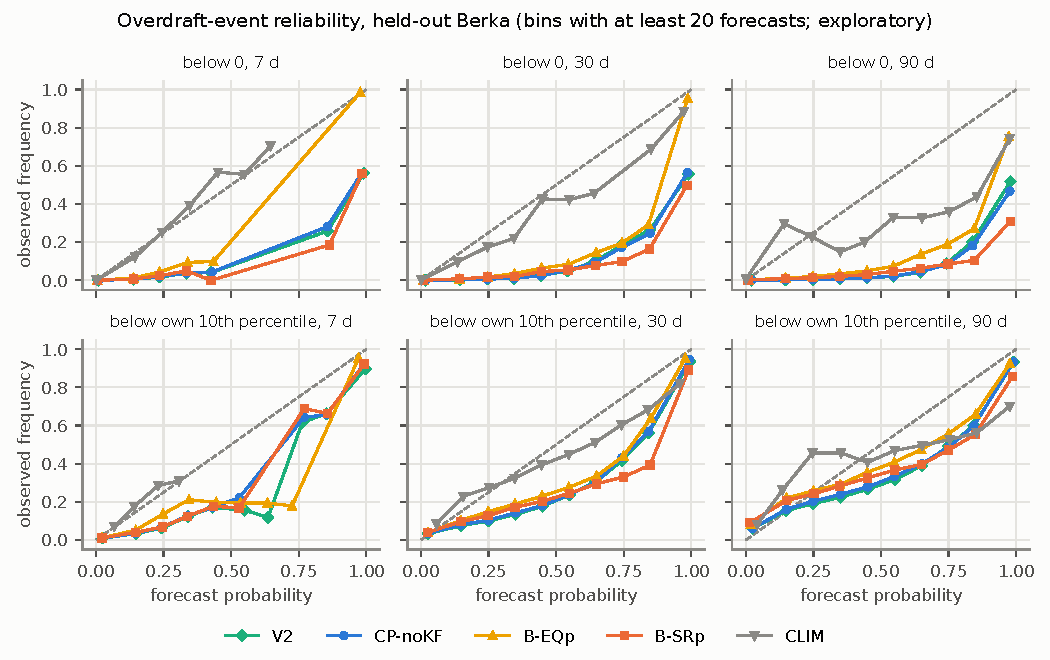
\includegraphics[width=\linewidth]{figures/overdraft-heldout.pdf}
\caption{Reliability of the overdraft-event probabilities on held-out Berka
(exploratory): observed frequency against forecast probability in ten
equal-width bins, shown where a bin holds at least twenty forecasts.
Below the diagonal: the method over-predicts the event. Bin counts are in
the exploratory held-out results.}
\label{fig:overdraft}
\end{figure}
